\documentclass[aspectratio=169]{beamer}

% Dependency setup
\usepackage{tikz}
%

% Beamer styling setup
\usetheme{AnnArbor}
\usecolortheme{beaver}
\setbeamercolor{titlelike}{parent=structure,bg=gray!15}
\setbeamertemplate{navigation symbols}{}
%

% Beamer notes setup
\usepackage{pgfpages}
\setbeameroption{show notes on second screen=right}
%

% Spacing setup
\setlength{\parindent}{0pt} % No paragraph indenting
\setlength{\parskip}{5pt} % Set spacing between paragraphs
\frenchspacing
\newcommand{\mkspace}{\vspace{19pt}}
\newcommand{\rmspace}{\vspace{-19pt}}
\newcommand{\emptyline}{\vspace{\baselineskip}}
%

\begin{document}
\title{Paraméteres bonyolultság}
\author{Kovács Milán, Nemkin Viktória}
\date{2021. március 16.}

\frame{\titlepage}

\frame{\frametitle{Menetrend}\tableofcontents}

\section{Motiváció}
\begin{frame}
\frametitle{Klasszikus bonyolultságelmélet}

Algoritmus: hány lépést tesz az input méretének függvényében?

\begin{itemize}
\item Nem biztos, hogy az egyforma méretű bemenetek egyformán nehezek...
\item Nem biztos, hogy egy teljesen általános megoldásra van szükségünk...
\end{itemize}

\end{frame}


\begin{frame}
\frametitle{Példa: Prímtényezős felbontás}

Feladat: prímtényezős felbontás megadása.
\emptyline

Kézzel melyiket lenne könnyebb megoldani?
\begin{itemize}
\item $4503599627370496 = 2^{52}$
\item $1125897758834689 = 524287 \cdot 2147483647$
\end{itemize}
\pause
Számítógépnek melyiket lenne könnyebb megoldani?
\begin{itemize}
\item 10000-nél kisebb prímszámok szorzata.
\item RSA kódolás feltörése: két nagyon nagy prím szorzatát felbontani.
\end{itemize}

\end{frame}


\begin{frame}
\begin{footnotesize}
\frametitle{Példa: Sűrű / ritka gráfok}
\note{Everything you want}

\begin{columns}
\begin{column}{0.5\textwidth}
Sűrű gráf:
\begin{center}
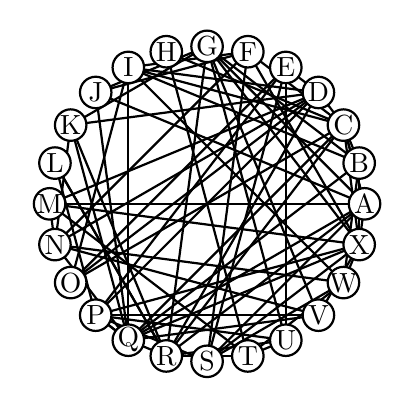
\begin{tikzpicture}[scale=2]
\coordinate (A) at (2.00000,1.00000);
\coordinate (B) at (1.96593,1.25882);
\coordinate (C) at (1.86603,1.50000);
\coordinate (D) at (1.70711,1.70711);
\coordinate (E) at (1.50000,1.86603);
\coordinate (F) at (1.25882,1.96593);
\coordinate (G) at (1.00000,2.00000);
\coordinate (H) at (0.74118,1.96593);
\coordinate (I) at (0.50000,1.86603);
\coordinate (J) at (0.29289,1.70711);
\coordinate (K) at (0.13397,1.50000);
\coordinate (L) at (0.03407,1.25882);
\coordinate (M) at (0.00000,1.00000);
\coordinate (N) at (0.03407,0.74118);
\coordinate (O) at (0.13397,0.50000);
\coordinate (P) at (0.29289,0.29289);
\coordinate (Q) at (0.50000,0.13397);
\coordinate (R) at (0.74118,0.03407);
\coordinate (S) at (1.00000,0.00000);
\coordinate (T) at (1.25882,0.03407);
\coordinate (U) at (1.50000,0.13397);
\coordinate (V) at (1.70711,0.29289);
\coordinate (W) at (1.86603,0.50000);
\coordinate (X) at (1.96593,0.74118);
\draw[thick] (B) -- (Q);
\draw[thick] (G) -- (V);
\draw[thick] (R) -- (U);
\draw[thick] (M) -- (X);
\draw[thick] (P) -- (P);
\draw[thick] (G) -- (U);
\draw[thick] (N) -- (M);
\draw[thick] (B) -- (I);
\draw[thick] (F) -- (N);
\draw[thick] (Q) -- (N);
\draw[thick] (A) -- (S);
\draw[thick] (N) -- (V);
\draw[thick] (X) -- (B);
\draw[thick] (B) -- (X);
\draw[thick] (J) -- (A);
\draw[thick] (T) -- (R);
\draw[thick] (F) -- (X);
\draw[thick] (N) -- (W);
\draw[thick] (V) -- (Q);
\draw[thick] (Q) -- (C);
\draw[thick] (R) -- (G);
\draw[thick] (Q) -- (R);
\draw[thick] (J) -- (F);
\draw[thick] (M) -- (D);
\draw[thick] (C) -- (H);
\draw[thick] (G) -- (A);
\draw[thick] (T) -- (U);
\draw[thick] (P) -- (Q);
\draw[thick] (H) -- (T);
\draw[thick] (P) -- (U);
\draw[thick] (C) -- (D);
\draw[thick] (S) -- (X);
\draw[thick] (S) -- (F);
\draw[thick] (X) -- (A);
\draw[thick] (I) -- (W);
\draw[thick] (I) -- (O);
\draw[thick] (I) -- (Q);
\draw[thick] (A) -- (C);
\draw[thick] (D) -- (O);
\draw[thick] (C) -- (A);
\draw[thick] (G) -- (J);
\draw[thick] (V) -- (X);
\draw[thick] (I) -- (D);
\draw[thick] (R) -- (D);
\draw[thick] (R) -- (C);
\draw[thick] (O) -- (E);
\draw[thick] (L) -- (P);
\draw[thick] (L) -- (R);
\draw[thick] (Q) -- (X);
\draw[thick] (W) -- (T);
\draw[thick] (E) -- (P);
\draw[thick] (K) -- (R);
\draw[thick] (S) -- (P);
\draw[thick] (U) -- (E);
\draw[thick] (V) -- (P);
\draw[thick] (R) -- (R);
\draw[thick] (E) -- (D);
\draw[thick] (B) -- (G);
\draw[thick] (M) -- (T);
\draw[thick] (N) -- (D);
\draw[thick] (D) -- (K);
\draw[thick] (X) -- (C);
\draw[thick] (C) -- (I);
\draw[thick] (N) -- (K);
\draw[thick] (A) -- (Q);
\draw[thick] (G) -- (X);
\draw[thick] (E) -- (S);
\draw[thick] (M) -- (A);
\draw[thick] (P) -- (X);
\draw[thick] (W) -- (S);
\draw[thick] (F) -- (I);
\draw[thick] (M) -- (M);
\draw[thick] (R) -- (A);
\draw[thick] (Q) -- (K);
\draw[thick] (R) -- (L);
\draw[thick] (Q) -- (P);
\draw[thick] (J) -- (Q);
\draw[thick] (P) -- (D);
\draw[thick] (G) -- (K);
\draw[thick] (W) -- (X);
\draw[thick] (C) -- (B);
\draw[thick] (W) -- (W);
\draw[thick] (F) -- (C);
\draw[thick] (O) -- (C);
\draw[thick] (H) -- (H);
\draw[thick] (W) -- (B);
\draw[thick, fill=white] (A) circle (0.1) node {A};
\draw[thick, fill=white] (B) circle (0.1) node {B};
\draw[thick, fill=white] (C) circle (0.1) node {C};
\draw[thick, fill=white] (D) circle (0.1) node {D};
\draw[thick, fill=white] (E) circle (0.1) node {E};
\draw[thick, fill=white] (F) circle (0.1) node {F};
\draw[thick, fill=white] (G) circle (0.1) node {G};
\draw[thick, fill=white] (H) circle (0.1) node {H};
\draw[thick, fill=white] (I) circle (0.1) node {I};
\draw[thick, fill=white] (J) circle (0.1) node {J};
\draw[thick, fill=white] (K) circle (0.1) node {K};
\draw[thick, fill=white] (L) circle (0.1) node {L};
\draw[thick, fill=white] (M) circle (0.1) node {M};
\draw[thick, fill=white] (N) circle (0.1) node {N};
\draw[thick, fill=white] (O) circle (0.1) node {O};
\draw[thick, fill=white] (P) circle (0.1) node {P};
\draw[thick, fill=white] (Q) circle (0.1) node {Q};
\draw[thick, fill=white] (R) circle (0.1) node {R};
\draw[thick, fill=white] (S) circle (0.1) node {S};
\draw[thick, fill=white] (T) circle (0.1) node {T};
\draw[thick, fill=white] (U) circle (0.1) node {U};
\draw[thick, fill=white] (V) circle (0.1) node {V};
\draw[thick, fill=white] (W) circle (0.1) node {W};
\draw[thick, fill=white] (X) circle (0.1) node {X};
\end{tikzpicture}
\end{center}

\end{column}

\begin{column}{0.5\textwidth}
Ritka gráf:
\begin{center}
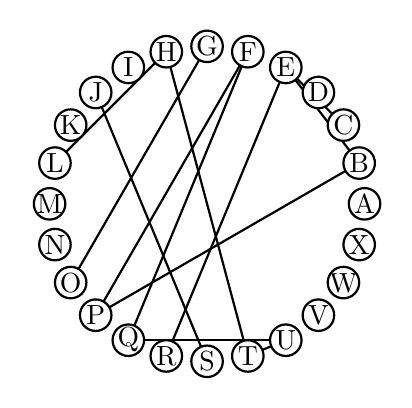
\begin{tikzpicture}[scale=2]
\coordinate (A) at (2.00000,1.00000);
\coordinate (B) at (1.96593,1.25882);
\coordinate (C) at (1.86603,1.50000);
\coordinate (D) at (1.70711,1.70711);
\coordinate (E) at (1.50000,1.86603);
\coordinate (F) at (1.25882,1.96593);
\coordinate (G) at (1.00000,2.00000);
\coordinate (H) at (0.74118,1.96593);
\coordinate (I) at (0.50000,1.86603);
\coordinate (J) at (0.29289,1.70711);
\coordinate (K) at (0.13397,1.50000);
\coordinate (L) at (0.03407,1.25882);
\coordinate (M) at (0.00000,1.00000);
\coordinate (N) at (0.03407,0.74118);
\coordinate (O) at (0.13397,0.50000);
\coordinate (P) at (0.29289,0.29289);
\coordinate (Q) at (0.50000,0.13397);
\coordinate (R) at (0.74118,0.03407);
\coordinate (S) at (1.00000,0.00000);
\coordinate (T) at (1.25882,0.03407);
\coordinate (U) at (1.50000,0.13397);
\coordinate (V) at (1.70711,0.29289);
\coordinate (W) at (1.86603,0.50000);
\coordinate (X) at (1.96593,0.74118);
\draw[thick] (T) -- (H);
\draw[thick] (Q) -- (U);
\draw[thick] (P) -- (F);
\draw[thick] (S) -- (J);
\draw[thick] (C) -- (E);
\draw[thick] (B) -- (P);
\draw[thick] (G) -- (O);
\draw[thick] (Q) -- (F);
\draw[thick] (E) -- (B);
\draw[thick] (H) -- (L);
\draw[thick] (E) -- (R);
\draw[thick] (T) -- (U);
\draw[thick, fill=white] (A) circle (0.1) node {A};
\draw[thick, fill=white] (B) circle (0.1) node {B};
\draw[thick, fill=white] (C) circle (0.1) node {C};
\draw[thick, fill=white] (D) circle (0.1) node {D};
\draw[thick, fill=white] (E) circle (0.1) node {E};
\draw[thick, fill=white] (F) circle (0.1) node {F};
\draw[thick, fill=white] (G) circle (0.1) node {G};
\draw[thick, fill=white] (H) circle (0.1) node {H};
\draw[thick, fill=white] (I) circle (0.1) node {I};
\draw[thick, fill=white] (J) circle (0.1) node {J};
\draw[thick, fill=white] (K) circle (0.1) node {K};
\draw[thick, fill=white] (L) circle (0.1) node {L};
\draw[thick, fill=white] (M) circle (0.1) node {M};
\draw[thick, fill=white] (N) circle (0.1) node {N};
\draw[thick, fill=white] (O) circle (0.1) node {O};
\draw[thick, fill=white] (P) circle (0.1) node {P};
\draw[thick, fill=white] (Q) circle (0.1) node {Q};
\draw[thick, fill=white] (R) circle (0.1) node {R};
\draw[thick, fill=white] (S) circle (0.1) node {S};
\draw[thick, fill=white] (T) circle (0.1) node {T};
\draw[thick, fill=white] (U) circle (0.1) node {U};
\draw[thick, fill=white] (V) circle (0.1) node {V};
\draw[thick, fill=white] (W) circle (0.1) node {W};
\draw[thick, fill=white] (X) circle (0.1) node {X};
\end{tikzpicture}
\end{center}

\end{column}
\end{columns}

\begin{itemize}
\item Input: szomszédossági mátrix $\rightarrow$ ugyanakkora.
\item Gráfalgoritmusok: független csúcshalmaz, klikk, színezés $\rightarrow$ nem egyformán nehéz.
\end{itemize}

\end{footnotesize}
\end{frame}


\begin{frame}
\frametitle{Valós életbeli problémák}

Üzleti korlátok:

\begin{itemize}
\item Facebook:
\begin{itemize}
\item ismerősök száma $\leq{}$ 500 (fokszám)
\item aktív felhasználók száma $\leq{}$ 3 milliárd (csúcsszám)
\end{itemize}
\item Google:
\begin{itemize}
\item keresett kifejezés hossza $\leq{}$ 100 karakter (illesztett minta hossza)
\item egy oldalon a linkek száma $\leq{}$ 1000 (fokszám)
\end{itemize}
\item Orvosi alkalmazások:
\begin{itemize}
\item DNS hosszúsága
\item protein max mérete
\end{itemize}
\end{itemize}
...stb
\end{frame}




\section{Bar Fight Prevention problem}
\begin{frame}
\frametitle{Feladat}

Sztori
\begin{itemize}
\item Biztonsági őr egy vidéki bárban
\item Péntek esti bulik: verekedés
\item Falu lakóit ismerjük, tudjuk ki kit nem szeret $\rightarrow$ ők verekedni fognak
\item Megelőzés: nem engedünk be olyanokat akik nem szeretik egymást
\item Menedzsment: profitmaximalizálás $\rightarrow$ legfeljebb k vendég elutasítása
\end{itemize}

Input
\begin{itemize}
\item Vendégek listája (n darab vendég)
\item Minden vendégpárra: szeretik-e egymást
\item Legfeljebb hány vendéget utasíthatunk el: k (kevesebbet lehet).
\end{itemize}

Output
\begin{itemize}
\item Megoldható-e úgy a feladat, hogy a beengedettek között ne legyen verekedés?
\item Kiket kell kitiltani?
\end{itemize}

\end{frame}


\begin{frame}
\frametitle{Megoldás}

\begin{center}
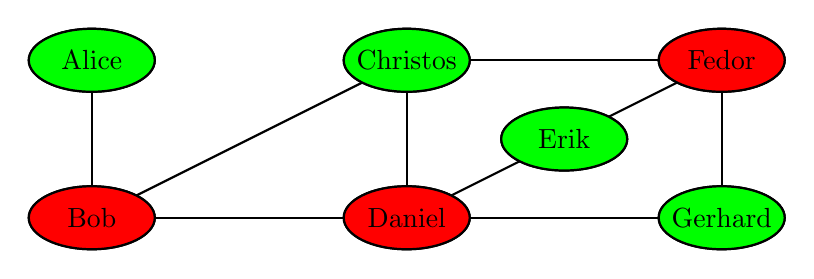
\begin{tikzpicture}[scale=2]
\coordinate (A) at (1,2);
\coordinate (B) at (1,1);
\coordinate (C) at (3,2);
\coordinate (D) at (3,1);
\coordinate (E) at (4,1.5);
\coordinate (F) at (5,2);
\coordinate (G) at (5,1);

\draw[thick] (B) -- (D);
\draw[thick] (D) -- (G);
\draw[thick] (C) -- (F);

\draw[thick] (B) -- (A);
\draw[thick] (D) -- (C);
\draw[thick] (G) -- (F);

\draw[thick] (B) -- (C);
\draw[thick] (D) -- (E);
\draw[thick] (E) -- (F);

\uncover<1>{\draw[thick, fill=white] (A) ellipse (0.4 and 0.2) node {Alice};}
\uncover<2>{\draw[thick, fill=green] (A) ellipse (0.4 and 0.2) node {Alice};}

\uncover<1>{\draw[thick, fill=white] (B) ellipse (0.4 and 0.2) node {Bob};}
\uncover<2>{\draw[thick, fill=red  ] (B) ellipse (0.4 and 0.2) node {Bob};}

\uncover<1>{\draw[thick, fill=white] (C) ellipse (0.4 and 0.2) node {Christos};}
\uncover<2>{\draw[thick, fill=green] (C) ellipse (0.4 and 0.2) node {Christos};}

\uncover<1>{\draw[thick, fill=white] (D) ellipse (0.4 and 0.2) node {Daniel};}
\uncover<2>{\draw[thick, fill=red  ] (D) ellipse (0.4 and 0.2) node {Daniel};}

\uncover<1>{\draw[thick, fill=white] (E) ellipse (0.4 and 0.2) node {Erik};}
\uncover<2>{\draw[thick, fill=green] (E) ellipse (0.4 and 0.2) node {Erik};}

\uncover<1>{\draw[thick, fill=white] (F) ellipse (0.4 and 0.2) node {Fedor};}
\uncover<2>{\draw[thick, fill=red  ] (F) ellipse (0.4 and 0.2) node {Fedor};}

\uncover<1>{\draw[thick, fill=white] (G) ellipse (0.4 and 0.2) node {Gerhard};}
\uncover<2>{\draw[thick, fill=green] (G) ellipse (0.4 and 0.2) node {Gerhard};}

\end{tikzpicture}
\end{center}

\begin{footnotesize}
\begin{itemize}
\item Csúcsok = vendégek, élek = verekedni fognak.
\item Kitilható vendégek száma: k=3.
\end{itemize}
Kérdések:
\begin{itemize}
\item Kit tiltsunk ki, hogy ne legyen verekedés? \\
\uncover<2>{\textcolor{red}{Bob-ot, Daniel-t és Fedor-t.}}
\item Melyik Algoritmuselméletből tanult feladat ez? \\
\uncover<2>{\textcolor{red}{Lefogó csúcshalmaz: $\forall$ él legalább egyik végpontja benne van.}}
\end{itemize}
\end{footnotesize}
\end{frame}


\begin{frame}
\frametitle{Megoldás}

\begin{center}
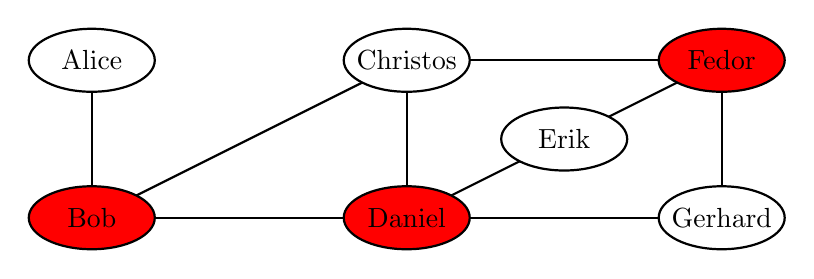
\begin{tikzpicture}[scale=2]
\coordinate (A) at (1,2);
\coordinate (B) at (1,1);
\coordinate (C) at (3,2);
\coordinate (D) at (3,1);
\coordinate (E) at (4,1.5);
\coordinate (F) at (5,2);
\coordinate (G) at (5,1);

\draw[thick] (B) -- (D);
\draw[thick] (D) -- (G);
\draw[thick] (C) -- (F);

\draw[thick] (B) -- (A);
\draw[thick] (D) -- (C);
\draw[thick] (G) -- (F);

\draw[thick] (B) -- (C);
\draw[thick] (D) -- (E);
\draw[thick] (E) -- (F);

\draw[thick, fill=white] (A) ellipse (0.4 and 0.2) node {Alice};
\draw[thick, fill=red  ] (B) ellipse (0.4 and 0.2) node {Bob};
\draw[thick, fill=white] (C) ellipse (0.4 and 0.2) node {Christos};
\draw[thick, fill=red  ] (D) ellipse (0.4 and 0.2) node {Daniel};
\draw[thick, fill=white] (E) ellipse (0.4 and 0.2) node {Erik};
\draw[thick, fill=red  ] (F) ellipse (0.4 and 0.2) node {Fedor};
\draw[thick, fill=white] (G) ellipse (0.4 and 0.2) node {Gerhard};
\end{tikzpicture}
\end{center}

\begin{footnotesize}
\begin{itemize}
\item Csúcsok = vendégek, élek = verekedni fognak.
\item Kitilható vendégek száma: k=3.
\end{itemize}
Kérdések:
\begin{itemize}
\item Kit tiltsunk ki, hogy ne legyen verekedés? \\
\textcolor{red}{Bob-ot, Daniel-t és Fedor-t.}
\item Melyik Algoritmuselméletből tanult feladat ez? \\
\textcolor{red}{Lefogó csúcshalmaz: $\forall$ él legalább egyik végpontja benne van.}
\end{itemize}
\end{footnotesize}
\end{frame}


\begin{frame}
\frametitle{Brute force megoldás}

\begin{footnotesize}
\begin{itemize}
\item Csúcsok száma: $n$ (pl. $1000$)
\item Kizárható emberek száma: $k$ (pl. $10$)
\end{itemize}
\end{footnotesize}

\begin{footnotesize}
\renewcommand{\arraystretch}{1.2}
\begin{center}
\begin{tabular}{ l | l | l }
Módszer & Lépések száma & Másodpercben ($10^8$ IPS) \\
\hline
\hline
Minden részhalmaz &
$2^n = 2^{1000} \approx 1.07\cdot10^{301}$ &
$1.07\cdot10^{293}$ $\rightarrow$ Univerzum életkora: $6.62\cdot10^{14}$ mp\\
\hline
Csak k elemű részhalmazok &
${{n}\choose{k}} = {{1000}\choose{10}} \approx 2.63\cdot10^{23}$ &
$2.63\cdot10^{15}$ $\rightarrow$ Nap hossza: $8.64\cdot10^{4}$ mp\\
\end{tabular}
\end{center}
\renewcommand{\arraystretch}{1}
\end{footnotesize}

Üzleti korlát: a menedzsment nem fog nagy $k$-t engedélyezni.

\end{frame}


\begin{frame}
\frametitle{Paraméter választás\uncover<2>{: fokszám}}

\begin{columns}
\begin{column}{0.5\textwidth}
\begin{footnotesize}
\begin{itemize}
\item Csúcsok száma: $n$ (pl. $1000$)
\item
\only<1>{Kizárható vendégek száma: $k$ (pl. $10$)}
\only<2>{\textcolor{red}{Még kizárható vendégek száma: $k'\leq{}k$ (pl. $10$)}}
\uncover<2>{\item\textcolor{red}{Csúcsok fokszáma: $1\leq{}d(v)\leq{}k'$}}
\end{itemize}
\emptyline
Mit tehetünk a következő csúcsokkal?
\begin{itemize}
\item A: $0$ fokszámú csúcs\\
\uncover<2>{\footnotesize{\textcolor{red}{$\rightarrow$ Beengedhető, nem ronthatja el}}}
\item B: $k+1\leq$ fokszámú csúcs\\
\uncover<2>{\footnotesize{\textcolor{red}{$\rightarrow$ Mindenképp ki kell zárni}}}\\
\uncover<2>{\footnotesize{\textcolor{red}{$\rightarrow$ k' = k-1 kizárás maradt}}}
\end{itemize}
\end{footnotesize}
\end{column}

\begin{column}{0.5\textwidth}
\begin{center}
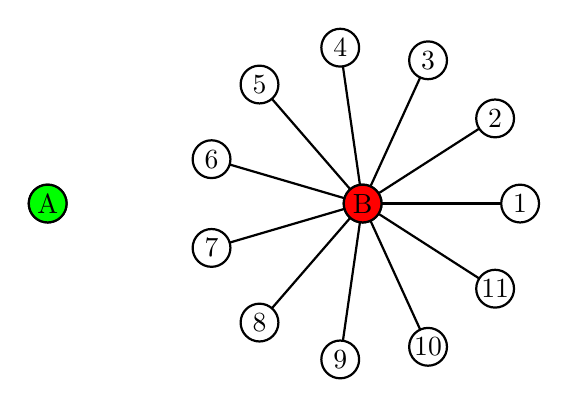
\begin{tikzpicture}[scale=2]
\coordinate (N1)  at (3.00000,1.00000);
\coordinate (N2)  at (2.84125,1.54064);
\coordinate (N3)  at (2.41542,1.90963);
\coordinate (N4)  at (1.85769,1.98982);
\coordinate (N5)  at (1.34514,1.75575);
\coordinate (N6)  at (1.04051,1.28173);
\coordinate (N7)  at (1.04051,0.71827);
\coordinate (N8)  at (1.34514,0.24425);
\coordinate (N9)  at (1.85769,0.01018);
\coordinate (N10) at (2.41542,0.09037);
\coordinate (N11) at (2.84125,0.45936);
\coordinate (A)   at (0.00000,1.00000);
\coordinate (B)   at (2.00000,1.00000);
\draw[thick] (B) -- (N1);
\draw[thick] (B) -- (N2);
\draw[thick] (B) -- (N3);
\draw[thick] (B) -- (N4);
\draw[thick] (B) -- (N5);
\draw[thick] (B) -- (N6);
\draw[thick] (B) -- (N7);
\draw[thick] (B) -- (N8);
\draw[thick] (B) -- (N9);
\draw[thick] (B) -- (N10);
\draw[thick] (B) -- (N11);
\draw[thick, fill=white] (N1)  circle (0.12) node{1};
\draw[thick, fill=white] (N2)  circle (0.12) node{2};
\draw[thick, fill=white] (N3)  circle (0.12) node{3};
\draw[thick, fill=white] (N4)  circle (0.12) node{4};
\draw[thick, fill=white] (N5)  circle (0.12) node{5};
\draw[thick, fill=white] (N6)  circle (0.12) node{6};
\draw[thick, fill=white] (N7)  circle (0.12) node{7};
\draw[thick, fill=white] (N8)  circle (0.12) node{8};
\draw[thick, fill=white] (N9)  circle (0.12) node{9};
\draw[thick, fill=white] (N10) circle (0.12) node{10};
\draw[thick, fill=white] (N11) circle (0.12) node{11};
\uncover<1>{\draw[thick, fill=white] (A)   circle (0.12) node {A};}
\uncover<2>{\draw[thick, fill=green] (A)   circle (0.12) node {A};}
\uncover<1>{\draw[thick, fill=white] (B)   circle (0.12) node {B};}
\uncover<2>{\draw[thick, fill=red]   (B)   circle (0.12) node {B};}
\end{tikzpicture}
\end{center}
\end{column}
\end{columns}

\end{frame}


\begin{frame}
\frametitle{Maradék gráf}

\begin{footnotesize}
\begin{itemize}
\item Csúcsok száma: $n$ (pl. $1000$)
\item Kizárható emberek száma: $k$ (pl. $10$)
\item Csúcsok fokszáma: $1\leq{}d(v)\leq{}k$
\end{itemize}
\end{footnotesize}

\begin{itemize}
\item Maradék gráf: 1...k fokú csúcsok. Minden kitiltás így k vagy kevesebb konfliktust fog megoldani a továbbiakban.
\item Ha több mint $k^2$ élünk van akkor biztosan nem megoldható a feladat, készen vagyunk.
\item Ha $k^2$ vagy kevesebb élünk van, akkor legfeljebb $2k^2$ csúcsunk lehet (minden élnek két vége van és nincs 0 fokú csúcs).
\item ${2k^2 \choose k}$ mostmár $k\leq{}10$-re már jobb mint az előbbi $2^n$.
\end{itemize}
\end{frame}

\input{02_bar_fight_prevention_problem/07_1_k_foku_graf}
\begin{frame}
\frametitle{1 fokú csúcsok}
\begin{itemize}
\item Az 1 fokú csúcs és szomszédja esetében: ha beengedem a csúcsot akkor az 1 darab szomszédját nem engedhetem be.
\item Ezzel biztos nem lett rosszabb a helyzet, mert ha a csúcsot nem engedem be akkor a szomszédját beengedhetem, de annak még lehetnek egyéb szomszédjai is.
\item Ezért engedjük be az 1 fokú csúcsokat és tiltsuk ki a szomszédokat (ezzel k-t is csökkentsük 1-el).
\item Így mostmár 2..k konfliktus lehet.
\item Erre megint kiszámolom a max csúcsszámot, ez mostmár csak $k^2$, erre még jobb szám jön ki.
\end{itemize}
\end{frame}

\input{02_bar_fight_prevention_problem/09_1_fokszamu_valasz}
\input{02_bar_fight_prevention_problem/10_2_k_foku_graf}
\input{02_bar_fight_prevention_problem/11_bounded_search_tree}

\section{Definíciók}

\begin{frame}
\frametitle{?}
Itt van még a példának folytatása bounded search tree-kkel, de azt inkább Milánnak kellene elmondania.
\end{frame}

\begin{frame}
\frametitle{Kernelizációs technika általánosan}
\end{frame}


\begin{frame}
\frametitle{Vertex cover feladat megoldása egyben}
\end{frame}

\begin{frame}
\frametitle{Paraméteres komplexitás definíciója általánosan}
\end{frame}

\section{Feedback arc set}

\begin{frame}
\frametitle{Szemezgetés}
\end{frame}
\end{document}
